\documentclass[journal]{IEEEtran}

\usepackage{cite}
\usepackage{amsmath}
\usepackage{amssymb}
\usepackage{graphicx}
\usepackage{booktabs}
\usepackage{array}
\usepackage{algorithm}
\usepackage{algpseudocode}
\usepackage{url}
\usepackage[hidelinks]{hyperref}

\begin{document}

\title{Do Hybrid Decision Tree--Na\"ive Bayes Gains Survive Leakage-Safe Evaluation?\\
A Replication of Farid et al.\ (2014)}

\author{First~A.~Author%
  \thanks{Manuscript received September 25, 2026. This work was carried out
  independently; affiliation placeholder.}%
  \markboth{Journal Name Placeholder,~Vol.~XX, No.~X, 2026}{Author: Do Hybrid DT--NB Gains Survive Leakage-Safe Evaluation?}}

\maketitle

\begin{abstract}
Farid et al.\ (2014) reported that a Na\"ive Bayes (NB) instance filter grown
into a decision tree, and a decision tree that weights attributes for NB,
each beat their base classifier on ten benchmark datasets. We replicate both
hybrids with the paper's own components (Weka J48 (pruned) and a
textbook NB on the original attribute columns) and test two evaluation
protocols: protocol A, in which the filter or the attribute weights are
fitted once on the whole dataset before cross-validation, and protocol B,
in which every stage is refit inside each training fold. The C4.5 baseline
is within 1.4 points of the paper on 7 of the 9 datasets other than NSL-KDD
and NB is within 2 points on 7 of 10; NSL-KDD is an unresolved outlier for
C4.5 (99.47\% here vs.\ 71.11\% reported). Under protocol B, Algorithm 1
reaches 81.02\% against a reported 88.43\%, and Algorithm 2 reaches 77.16\%
against a reported 83.42\%. Protocol A inflates Algorithm 1 by a median of 11.58 points
(Wilcoxon $W$=0, $p$=0.002, Holm-adjusted $p$=0.016, $n$=10 datasets) and
Algorithm 2 by a median of only 0.14 points ($p$=0.164, not significant after
correction). A second, independent codebase (sklearn CART, one-hot
attributes) reproduces the same pattern (mean inflation +15.57 vs.\ +0.78 points). Under refit-per-fold
evaluation neither hybrid shows a significant gain over its base classifier,
and swapping the order of the two algorithms changes mean accuracy by less
than one point. We
report these results as preliminary (3 and 5 seeds) and discuss what the
audit does and does not establish.
\end{abstract}

\begin{IEEEkeywords}
decision tree, Na\"ive Bayes, hybrid classifier, data leakage, cross-validation,
replication study, noise filtering, attribute weighting
\end{IEEEkeywords}

\IEEEpeerreviewmaketitle

\section{Introduction}

\IEEEPARstart{D}{ecision} trees and Na\"ive Bayes are two of the oldest
workhorses of supervised classification, and each covers the other's
weak spot: a tree splits on whichever attribute looks most informative at
each node but ignores the rest of the joint distribution, while NB uses
every attribute but assumes they are independent given the class. Farid
et al.~\cite{farid2014hybrid} proposed two hybrids that combine the two
models in opposite directions. Algorithm 1 trains a NB classifier, uses it
to flag the training instances it misclassifies as noise, deletes them,
and grows a C4.5 tree on what remains. Algorithm 2 grows a tree first,
turns the depth at which each attribute is tested into a weight
($1/\sqrt{d}$, zero for attributes the tree never tests), and plugs those
weights into NB's class-conditional likelihood. Both hybrids were reported
to outperform their un-hybridized counterpart on ten benchmark
datasets (nine from the UCI repository plus NSL-KDD), and the paper has since accumulated a substantial citation
record built on those numbers.

Three properties of the original evaluation raise concern independently
of whether the numbers are correct. First, the paper never states whether
the noise filter and the attribute weights were fit once on the full
dataset or refit inside each cross-validation fold; if it is the former,
every deleted instance and every attribute weight was chosen with
knowledge of the labels of the instances later used for testing, which is
exactly the kind of preprocessing leakage that inflates reported accuracy
in unrelated
domains~\cite{cawley2010overfitting,demircioglu2021measuring,kapoor2023leakage,bouke2023empirical}.
Second, Algorithm 1 equates ``the instance NB gets wrong'' with ``the
instance is noise,'' a design that later work on label-noise filtering
identifies as one of the weaker choices available, because a single model
is both the source and the arbiter of its own
disagreement~\cite{brodley1999identifying,jiang2024correction,northcutt2021confident}.
Third, the two hybrids were evaluated separately: nobody, including the
original paper, reports what happens when the filter and the weighting
scheme are chained, in either order, inside one pipeline.

This paper reports a replication built to check the first two concerns
directly and to measure the third. Our contributions are:
\begin{itemize}
\item \textbf{A faithful replication (R1)} of Farid et al.'s two hybrids
using the paper's own components (Weka J48 (pruned, default options) as
C4.5 and a textbook NB on the original nominal attribute columns) under
two evaluation protocols: protocol A (fit-before-CV), where the filter or
weights are fit once on the whole dataset, and protocol B
(refit-per-fold), where every stage is refit inside each training fold.
\item \textbf{A quantified leakage audit (E3a)} that isolates the effect of
protocol alone, holding the algorithms, data encoding and classifiers
fixed, and repeats the audit on an independent codebase (sklearn entropy
trees, one-hot attributes) to check the finding is not an artifact of one
implementation.
\item \textbf{A two-order pipeline study (E9)} that chains Algorithm 1 and
Algorithm 2 in both possible orders under protocol B, with a final NB or
decision tree, to measure whether order or combination changes the
honest picture.
\item \textbf{Honest statistical reporting} of every comparison as a
Wilcoxon signed-rank test over the ten datasets, Holm-adjusted, with an
explicit acknowledgment of the low power that ten paired
datasets gives~\cite{demsar2006statistical}.
\end{itemize}
All numbers in this paper are computed by a script from CSV files produced
by runnable code; none are transcribed from earlier notes or hand-copied
from the original paper's tables.

\section{Related Work}

Decision-tree/Na\"ive-Bayes hybrids predate Farid et al.'s paper by nearly
two decades. Kohavi's NBTree~\cite{kohavi1996scaling} grows a tree and
places a local NB classifier at each leaf, using the tree to partition the
instance space rather than to select or weight attributes. Closer to
Algorithm 2's mechanism, Hall~\cite{hall2007decision} weights each
attribute for NB by a function of the depth at which a decision tree
tests it, on the same reasoning Farid et al.\ use (attributes near the
root separate classes more cleanly and should count more) but the two
papers were developed independently and Farid et al.\ do not cite
Hall's. Algorithm 1's filter-then-grow design continues a line that goes
back to John's robust decision
trees~\cite{john1995robust}, which also delete training instances a
classifier misclassifies before regrowing a tree on the remainder; the
family shares the same basic assumption that disagreement with a fitted
model is a reasonable proxy for label noise.

That assumption is the most contested part of the noise-filtering
literature. Brodley and Friedl~\cite{brodley1999identifying} show that a
single classifier used as its own noise judge is the weakest filtering
design available, because its errors on ambiguous but correctly labeled
instances are indistinguishable from its errors on genuinely mislabeled
ones; ensemble and consensus filters are more conservative and better
calibrated. Wong et al.~\cite{wong2020instance} build a more recent
instance-filtering hybrid that outperforms earlier one-shot filters
including designs close to Algorithm 1, and confident-learning
methods~\cite{northcutt2021confident} replace hard deletion with an
estimated confidence score per instance so uncertain cases can be
downweighted rather than discarded. On the correction side, Jiang et
al.~\cite{jiang2024correction} report that correcting a mislabeled
instance's label is often more effective than removing the instance
outright, which is a direct critique of Algorithm 1's delete-only design.
On the attribute side, tree-derived weighting for NB has continued past
Hall's original scheme; Zhang et al.~\cite{zhang2023multiview} build a
multi-view attribute-weighted NB from an ensemble of random trees rather
than a single tree, trading Algorithm 2's simplicity for a less
variance-prone weight estimate. Whether instance and attribute operations
should run in a fixed order, and whether that order matters, has direct
evidence in two places: Tsai et al.~\cite{tsai2013genetic} use a genetic
algorithm to learn a priority between feature and instance selection and
find the priority itself affects accuracy, and S\'aez et
al.~\cite{saez2015smoteipf} show that running a noise filter before
resampling strips borderline minority instances that resampling after
filtering would have kept, a sharp demonstration that pipeline order is
not a free choice. Both motivate directly testing the two possible orders
of Algorithms 1 and 2 rather than assuming they commute, which is what
the E9 study in Section~\ref{sec:experiments} does.

The third relevant body of work is methodological rather than about
classifiers. Cawley and Talbot~\cite{cawley2010overfitting} give the
general argument that any model-selection or preprocessing step fit on
data that later contributes to the reported test score produces an
optimistically biased estimate, and prescribe nesting that step inside
cross-validation; this is precisely the choice Farid et al.'s protocol
never states, and precisely what protocols A and B in this paper are
designed to separate. Demircio\u{g}lu~\cite{demircioglu2021measuring}
quantifies the resulting bias in a medical-imaging setting at up to 0.15
AUC or 0.17 accuracy when feature selection is fit outside
cross-validation, worse as the ratio of samples to features shrinks, which
matches the small-sample, many-attribute character of several datasets
used here. Kapoor and Narayanan~\cite{kapoor2023leakage} survey the same
failure mode across machine-learning-based science broadly and argue it
is common enough to be a contributor to the field's reproducibility
problems, and Bouke and Abdullah~\cite{bouke2023empirical} demonstrate the
effect concretely on NSL-KDD, one of the ten datasets used in this
replication, which is one reason NSL-KDD receives separate attention in
Section~\ref{sec:results}.

\section{Background: Farid's Algorithms 1 and 2}
\label{sec:background}

This section restates the two algorithms as printed in
Farid et al.~\cite{farid2014hybrid} (Section 4, pp.~1941--1942), because
the replication in Section~\ref{sec:setup} depends on reproducing their
exact steps rather than a paraphrase of their intent.

\subsection{Algorithm 1: the hybrid decision tree}

Algorithm 1 first classifies every training instance with a NB classifier
fit on the same training data, using the standard class-conditional
probabilities $P(C_i)$ and $P(A_{ij}\mid C_i)$; every instance the NB
classifier misclassifies (its posterior-probability class disagrees with
the recorded label) is removed from the training set. A C4.5-style
decision tree is then grown on the reduced training set by ordinary
recursive splitting: pick the best splitting attribute, create a labeled
root, branch on each split predicate, and recurse until a stopping
criterion is met at each branch.

\begin{algorithm}[t]
\caption{Hybrid decision tree induction (Farid et al.~\cite{farid2014hybrid}, Alg.\ 1)}
\label{alg:1}
\begin{algorithmic}[1]
\Require Training dataset $D=\{x_1,\dots,x_n\}$ with class labels
\Ensure Decision tree $T$
\For{each class $C_i \in D$}
  \State find prior probability $P(C_i)$
\EndFor
\For{each attribute value $A_{ij} \in D$}
  \State find class-conditional probability $P(A_{ij}\mid C_i)$
\EndFor
\For{each training instance $x_i \in D$}
  \State find posterior probability $P(C_i\mid x_i)$
  \If{$x_i$ is misclassified}
    \State remove $x_i$ from $D$
  \EndIf
\EndFor
\State $T \gets \emptyset$; determine the best splitting attribute
\State create the root node of $T$, labeled with that attribute
\State add an arc to the root for each split predicate/label
\For{each arc}
  \State $D \gets$ the subset of $D$ that satisfies the arc's predicate
  \If{a stopping point is reached on this path}
    \State create a leaf labeled with the majority class
  \Else
    \State recursively build a subtree on $D$
  \EndIf
  \State attach the resulting subtree to the arc
\EndFor
\end{algorithmic}
\end{algorithm}

\subsection{Algorithm 2: the hybrid Na\"ive Bayes classifier}

Algorithm 2 reverses the order: a decision tree is grown first on the full
training set, by the same recursive splitting procedure as Algorithm~1's
second half. Every attribute the tree tests is then given a weight
$W_i = 1/\sqrt{d}$, where $d$ is the smallest depth (root $=1$) at which
the tree tests that attribute; an attribute the tree never tests gets
$W_i = 0$ and is dropped from the classifier entirely. A NB classifier is
then built using only the attributes with $W_i \neq 0$, with each
class-conditional probability raised to the power of its attribute's
weight:
\begin{equation}
P(x_i \mid C_i) = \prod_{j=1}^{n} P(A_{ij}\mid C_i)^{W_i}. \label{eq:14}
\end{equation}
Equation~\eqref{eq:14} is the paper's Eq.~(14); the posterior
$P(C_i\mid x_i)$ used for classification combines this weighted likelihood
with the class prior in the usual NB way.

\begin{algorithm}[t]
\caption{Hybrid Na\"ive Bayes classifier (Farid et al.~\cite{farid2014hybrid}, Alg.\ 2)}
\label{alg:2}
\begin{algorithmic}[1]
\Require Training dataset $D=\{x_1,\dots,x_n\}$ with class labels
\Ensure A NB classification model
\State build a decision tree $T$ on $D$ (as in Alg.~\ref{alg:1}, lines 9--16)
\For{each attribute $A_i \in D$}
  \If{$A_i$ is not tested in $T$}
    \State $W_i \gets 0$
  \Else
    \State $d \gets$ the smallest depth at which $T$ tests $A_i$
    \State $W_i \gets 1/\sqrt{d}$
  \EndIf
\EndFor
\For{each class $C_i \in D$}
  \State find prior probability $P(C_i)$
\EndFor
\For{each attribute $A_i \in D$ with $W_i \neq 0$}
  \For{each value $A_{ij}$ of $A_i$}
    \State find $P(A_{ij}\mid C_i)$
  \EndFor
\EndFor
\For{each instance $x_i \in D$}
  \State find posterior probability $P(C_i\mid x_i)$ using Eq.~\eqref{eq:14}
\EndFor
\end{algorithmic}
\end{algorithm}

Two properties of these algorithms matter for what follows. First, neither
step in Algorithm~1 or Algorithm~2 is stated as being confined to a
training fold; the paper's description is silent on whether the filter or
the tree ever sees an instance that is later scored as a test case. Second,
Algorithm 1's notion of noise is entirely internal to one NB fit: an
instance is noise if and only if this particular classifier, trained on
this particular data, disagrees with its label, with no second opinion and
no confidence threshold.

\section{Replication Setup and Protocols}
\label{sec:setup}

\subsection{Datasets}

We use the same ten datasets as Farid et al.'s Table 5: breast cancer,
contact lenses, diabetes, glass, iris, soybean, vote, image segmentation,
tic-tac-toe, and NSL-KDD~\cite{tavallaee2009detailed}. NSL-KDD is the
corrected, de-duplicated successor to KDD Cup 1999 and is the one dataset
in the set built specifically to study intrusion-detection classifiers
rather than as a generic UCI benchmark; it is also the dataset on which a
preprocessing-leakage effect has previously been
documented~\cite{bouke2023empirical}, which is one reason its results are
reported separately rather than folded into an average.

\subsection{Two evaluation protocols}

Every experiment in this paper compares the same two protocols, applied to
whichever stages an arm uses (the NB filter of Algorithm~1, the tree-based
attribute weighting of Algorithm~2, or both):
\begin{itemize}
\item \textbf{Protocol B (refit-per-fold, honest).} For each of the 10
cross-validation folds, every stage (the filter, the attribute
selector, and the final classifier) is fit on that fold's training
split only, and scored on that fold's held-out test split. No stage ever
sees a label from a test instance before that instance is scored.
\item \textbf{Protocol A (fit-before-CV).} The filter and/or the attribute
selector are fit once on the entire dataset, using every instance's label.
Cross-validation is then run only over the final classifier, on the data
already cleaned or reduced by that one full-data fit. This is the protocol
consistent with a plain reading of Farid et al.'s Section 4, which never
mentions folds when it describes Algorithms 1 and 2, and only introduces
10-fold cross-validation afterward, in Section 5, as the way the resulting
classifier is scored.
\end{itemize}
Where a fully leaky upper bound is useful for calibration, we also report
\textbf{protocol C}: the stages and the final classifier are fit on the
whole dataset and then scored on that same data, with no held-out split at
all. Protocol C is not a protocol anyone would defend; it exists only to
show how high a number leakage can reach.

\subsection{R1: faithful replication with the paper's own components}

R1 reproduces Farid et al.'s Tables 8--11 as closely as the paper's own
tools allow. C4.5 is Weka J48 3.8.6~\cite{witten2016weka}, pruned, with
Weka's default options (\texttt{-C 0.25 -M 2}), matching Quinlan's original
C4.5~\cite{quinlan1993c45} far more closely than a CART-style tree does,
because J48 splits a nominal attribute into one branch per value rather
than into binary one-hot tests; this matters because Algorithm~2's notion
of ``the attribute'' and its minimum-depth weight are only meaningful in
the attribute space the paper used. NB is a from-scratch implementation
(add-one Laplace counts on nominal attributes, Gaussian likelihood on
numeric ones) fit on the datasets' original, non-one-hot columns, because
Weka's own NB diverges from this textbook form on attributes with very
wide numeric ranges such as NSL-KDD's byte counts. Algorithm~1 uses this
NB as its noise judge; Algorithm~2 uses J48's tree structure for the
minimum-depth weights and the same NB, weighted by Eq.~\eqref{eq:14}, as
its final classifier. Both protocols above are run for every arm, with 3
seeds and stratified 10-fold cross-validation per seed. As a sensitivity
check, R1 is repeated once with J48 unpruned (\texttt{-U -M 2}).

\subsection{E3a: an independent leakage audit}

E3a re-runs the same protocol-A/B/C comparison with a second, independent
implementation: scikit-learn~\cite{pedregosa2011scikit} decision trees
grown with entropy splitting (CART, not C4.5), a one-hot encoding of
nominal attributes, and a NB with mixed likelihoods (Bernoulli on the
0/1 one-hot columns, Gaussian elsewhere). If the protocol-A inflation seen
in R1 were an artifact of the Weka/J48 implementation, it should not
reappear here; if it is a property of the algorithms and the leaky
protocol, it should. E3a uses 3 seeds and stratified 10-fold
cross-validation, tree pruning strength $\mathrm{ccp\_alpha}=0.01$.

\subsection{E9: the two orders of Algorithm 1 and Algorithm 2}

E9 chains Algorithm~1 (instance filtering, written $N$) and Algorithm~2
(attribute weighting, written $A$) in both possible orders, always under
protocol B: Path~1 is $N\to A$ (filter, then weight attributes on the
filtered rows), Path~2 is $A\to N$ (weight attributes, then filter
instances using the weighted NB as judge). Both paths end in either a
final NB or a final decision tree, alongside single-stage (Algorithm~1
alone, Algorithm~2 alone) and no-cleaning baseline arms, all evaluated on
the same folds so every arm is directly comparable. E9 uses the same
scikit-learn CART/one-hot/mixed-NB implementation as E3a, tree pruning
strength $\mathrm{ccp\_alpha}=0$ (no pruning), and Algorithm~2's weights
are also handed to Algorithm~1's judge and to the final NB when both
stages run. E9 uses 5 seeds and stratified 10-fold cross-validation.

\subsection{Statistical testing}

Every comparison in this paper is a Wilcoxon signed-rank test over the ten
datasets: for a given pair of conditions, the ten paired accuracy
differences (one per dataset, averaged over that condition's seeds and
folds already) are tested against a null median difference of zero,
two-sided, using SciPy. With only ten datasets, this gives $n=10$ paired
observations per test, which is a small sample by any standard and a low-power
test in the sense discussed by Dem\v{s}ar~\cite{demsar2006statistical};
we report the Wilcoxon statistic, the raw $p$-value, the median paired
difference, and a Holm step-down correction applied across the family of
eight tests reported in Table~\ref{tab:tests}, and we do not claim
significance where the corrected $p$-value does not support it. No
per-fold results are stored in the underlying CSV files, so no
resampled or corrected paired $t$-test is computed; only the
between-dataset Wilcoxon test is reported.

\section{Experiments}
\label{sec:experiments}

Given the setup in Section~\ref{sec:setup}, three experiments answer three
separate questions, each tested against a specific, falsifiable claim.

\textbf{R1} asks whether Farid et al.'s baselines and hybrids reproduce
under the paper's own components. It tests two claims: that the C4.5 and
NB baselines replicate closely (Section~\ref{sec:results} reports the
per-dataset gap to the paper's Tables 8--11), and that protocol A inflates
Algorithm~1 more than Algorithm~2, since Algorithm~1's filter removes rows
from the training set that a leaky protocol also removes from the test
folds, while Algorithm~2 only drops columns, which changes what a fold
learns from but not which instances a fold ever sees.

\textbf{E3a} asks whether the R1 inflation pattern is specific to the
Weka/J48 implementation or a property of the algorithms and the leaky
protocol in general, by repeating the same protocol-A-vs-B comparison with
an independent sklearn/one-hot/CART implementation. If both
implementations show the same asymmetry (large Algorithm~1 inflation,
small Algorithm~2 inflation), the asymmetry is attributable to the
algorithms' design, not to one toolchain.

\textbf{E9} asks two questions about the pipeline that Farid et al.\ never
built: whether either honest hybrid beats its non-hybrid baseline under
protocol B (Algorithm~1's tree vs.\ a plain tree; Algorithm~2's NB vs.\
plain NB), and whether the order in which the two algorithms are chained
(Path~1, filter-then-weight, vs.\ Path~2, weight-then-filter) changes
accuracy. E9 also records, per dataset, the percentage of training rows
Algorithm~1 removes and the percentage of attributes Algorithm~2 keeps, to
check whether a large removal or reduction predicts a large accuracy
change in the downstream classifier, which is the relationship plotted in
Fig.~\ref{fig:removal}.

All three experiments share the same ten datasets, the same protocol-B
refit-per-fold discipline as the default honest condition, and the same
Wilcoxon-over-datasets testing procedure described in
Section~\ref{sec:setup}. Table~\ref{tab:tests} collects every statistical
test from all three experiments in one place so the eight $p$-values can
be Holm-adjusted as one family rather than read as eight independent
tests.

\section{Results}
\label{sec:results}

\subsection{Baselines replicate; the hybrids do not}

Table~\ref{tab:r1} lists, for every dataset, the protocol-B (honest)
accuracy of the C4.5 and NB baselines and of Algorithms 1 and 2, next to
Farid et al.'s reported numbers. The C4.5 baseline is within 1.4 points of
the paper on 7 of the 9 non-NSL-KDD datasets (largest gap $-2.89$ on iris,
smallest 0.00 on diabetes), and the NB baseline is within 2.0 points on 7
of 10 datasets. NSL-KDD is the exception for C4.5: this replication scores
99.47\% against a reported 71.11\%, a 28.36-point gap far outside the
spread on any other dataset; we did not find a configuration change that
closes it and report it as unresolved rather than adjust the protocol
until it matches. The hybrids do not replicate on average: Algorithm~1
reaches a mean of 81.02\% against a reported 88.43\%, worst on glass
($-27.14$), and Algorithm~2 reaches 77.16\% against 83.42\%, worst on
NSL-KDD ($-19.66$). Table~\ref{tab:tests} shows neither honest hybrid
beats its baseline once Holm correction is applied: Algorithm~1 vs.\ C4.5
has a median difference of $-3.71$ points ($p=0.055$, Holm $p=0.328$), and
Algorithm~2 vs.\ NB has a median difference of $+0.65$ points ($p=0.164$,
Holm $p=0.656$). Neither result supports the paper's claim of a
consistent hybrid advantage under an evaluation protocol that never lets a
stage see a test instance's label.

% R1: Weka J48 (pruned) / FaithfulNB replication, protocol B honest, 10-fold CV x 3 seeds.
\begin{table*}[t]
\caption{R1 replication (protocol B, refit-per-fold): C4.5 and NB baselines and the two hybrids, against Farid et al.\ (2014).}
\label{tab:r1}
\centering\small
\begin{tabular}{lrrrrrrrr}
\toprule
& \multicolumn{2}{c}{C4.5} & \multicolumn{2}{c}{NB} & \multicolumn{2}{c}{Alg.\ 1} & \multicolumn{2}{c}{Alg.\ 2} \\
Dataset & ours & paper & ours & paper & ours & paper & ours & paper \\
\midrule
breast-cancer & 75.31 & 75.52 & 72.39 & 71.67 & 71.61 & 81.46 & 72.63 & 75.87 \\
contact-lenses & 85.00 & 83.33 & 73.33 & 70.83 & 85.00 & 91.66 & 79.44 & 87.50 \\
diabetes & 73.82 & 73.82 & 75.52 & 76.30 & 75.52 & 79.03 & 77.12 & 85.41 \\
glass & 66.88 & 66.82 & 46.60 & 48.59 & 49.13 & 76.27 & 47.41 & 52.33 \\
image-segmentation & 96.75 & 95.73 & 79.67 & 81.06 & 89.11 & 96.53 & 81.75 & 85.19 \\
iris & 93.11 & 96.00 & 95.56 & 96.00 & 94.67 & 98.66 & 95.56 & 98.00 \\
nsl-kdd & 99.47 & 71.11 & 67.44 & 76.27 & 86.57 & 81.92 & 62.73 & 82.39 \\
soybean & 92.54 & 91.50 & 89.94 & 92.83 & 88.82 & 92.97 & 89.40 & 94.15 \\
tic-tac-toe & 85.08 & 85.07 & 69.87 & 69.62 & 74.50 & 88.10 & 70.36 & 78.91 \\
vote & 94.93 & 96.32 & 90.18 & 90.11 & 95.25 & 97.70 & 95.24 & 94.48 \\
\bottomrule
\end{tabular}
\end{table*}


\subsection{Fitting the filter before cross-validation inflates Algorithm 1}

Table~\ref{tab:tests} reports the protocol-A-vs-B comparison directly.
Under R1's Weka/J48 implementation, moving Algorithm~1 from protocol B to
protocol A raises accuracy by a median of 11.58 points across the ten
datasets ($W=0$, $p=0.002$, Holm $p=0.016$): every one of the ten datasets
moves in the same direction, which is why the Wilcoxon statistic is at its
minimum possible value. Algorithm~2 moves by a median of only 0.14 points
under the same protocol change ($p=0.164$, Holm $p=0.656$, not
significant). The same asymmetry appears in E3a's independent
sklearn/one-hot/CART implementation (Table~\ref{tab:e3a}): Algorithm~1's
mean accuracy rises from 80.58\% (protocol B) to 96.16\% (protocol A), a
mean gap of $+15.57$ points, with the paired test again significant after
correction ($W=0$, $p=0.002$, Holm $p=0.016$, median $+15.52$); Algorithm~2
rises from 75.00\% to 75.78\%, a mean gap of only $+0.78$ points and not
significant ($p=0.129$, Holm $p=0.645$). The chained paths inflate by
similarly large amounts under protocol A (Path~1 ($N\to A$) by a mean
of $+16.42$ points and Path~2 ($A\to N$) by $+17.73$) because both
paths include Algorithm~1's filtering step. The mechanism is direct:
protocol A deletes, from the entire dataset, every instance the filter's
judge disagrees with, so those instances never appear in any test fold
either; since the deleted instances are disproportionately the ones a
model finds hard, removing them from the test side of every fold inflates
accuracy independently of anything protocol B's honest classifier
actually learned. Algorithm~2 only removes columns, which changes what
every fold's classifier is trained and tested on but does not remove any
row from any test fold, and its leakage is correspondingly close to zero
in both implementations. Fig.~\ref{fig:r1_protocols} shows this pattern
per dataset: the protocol-A bars for Algorithm~1 (bottom panel of the pair
is Algorithm~2) sit far above both the protocol-B bars and the paper's own
reported numbers on most datasets, while Algorithm~2's three series track
each other closely.

% E3a: sklearn entropy CART / one-hot / mixed-likelihood NB, protocol B honest vs A before-CV vs C fully leaky.
\begin{table}[t]
\caption{E3a leakage check, mean accuracy over 10 datasets (entropy CART, one-hot attributes, mixed-likelihood NB).}
\label{tab:e3a}
\centering\small
\setlength{\tabcolsep}{3pt}
\begin{tabular}{lrrrr}
\toprule
Arm & B honest & A before-CV & C on all data & A$-$B \\
\midrule
baseline (NB) & 77.96 & 77.96 & 79.26 & +0.00 \\
baseline (DT) & 84.81 & 84.81 & 99.78 & +0.00 \\
Alg1 & 80.58 & 96.16 & 100.00 & +15.57 \\
Alg2 & 75.00 & 75.78 & 78.72 & +0.78 \\
C1 N->A & 80.39 & 96.81 & 99.91 & +16.42 \\
C2 A->N & 79.41 & 97.15 & 100.00 & +17.73 \\
\bottomrule
\end{tabular}
\end{table}


\begin{figure}[t]
\centering
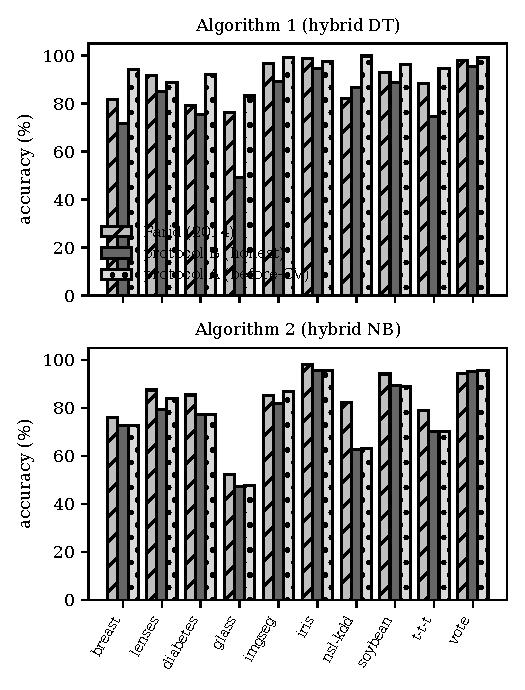
\includegraphics[width=3.4in]{figures/fig1_r1_protocols.pdf}
\caption{Accuracy of Algorithm~1 (top) and Algorithm~2 (bottom) per
dataset: Farid et al.'s reported number, protocol B (refit-per-fold,
honest), and protocol A (fit-before-CV). Algorithm~1's protocol-A bars are
inflated on almost every dataset; Algorithm~2's three series stay close
together.}
\label{fig:r1_protocols}
\end{figure}

\subsection{The filter hurts a downstream tree, and order barely matters}

Table~\ref{tab:e9} reports E9's protocol-B pipeline results. Chaining
Algorithm~1 into a final tree costs accuracy relative to the no-cleaning
baseline (80.58\% vs.\ 85.16\% mean, both final DT), and the cost is not
uniform across datasets: Fig.~\ref{fig:removal} plots, per dataset, the
percentage of training rows Algorithm~1 removes against the resulting
change in the tree's accuracy relative to the baseline tree. The largest
drop is on tic-tac-toe ($-18.18$ points), and the only clear gain is on
breast-cancer ($+5.45$ points), consistent with a filter that helps only
where the NB judge is a better error detector than the tree already is on
its own, and otherwise discards rows the tree needed. Algorithm~2's effect
on the tree is close to neutral (85.01\% vs.\ 85.16\%), consistent with a
tree re-deriving similar splits from whichever 69.97\% of attributes
survive selection on average. Swapping the order of the two algorithms
changes accuracy by less than one point on both final classifiers: Path~2
minus Path~1 has a median difference of $-0.09$ points for a final tree
($p=0.846$) and $+0.97$ points for a final NB ($p=0.322$), neither
significant even before correction. Order is not the lever that recovers
the paper's reported gains.

% E9: refit-per-fold, 10-fold CV x 5 seeds, alpha=0, mixed NB, weights on.
\begin{table}[t]
\caption{E9 pipeline, mean accuracy over 10 datasets ($\pm$ across-dataset SD), 10-fold CV $\times$ 5 seeds.}
\label{tab:e9}
\centering\small
\begin{tabular}{lrr}
\toprule
Arm & final DT & final NB \\
\midrule
baseline (no cleaning) & 85.16 $\pm$ 13.42 & 77.82 $\pm$ 14.13 \\
Algorithm 1 alone & 80.58 $\pm$ 13.41 & 76.58 $\pm$ 16.38 \\
Algorithm 2 alone & 85.01 $\pm$ 13.38 & 76.45 $\pm$ 14.33 \\
Path 1 (Alg1 $\to$ Alg2) & 80.52 $\pm$ 13.49 & 76.15 $\pm$ 16.70 \\
Path 2 (Alg2 $\to$ Alg1) & 79.54 $\pm$ 14.09 & 75.89 $\pm$ 14.77 \\
\bottomrule
\end{tabular}
\end{table}


\begin{figure}[t]
\centering
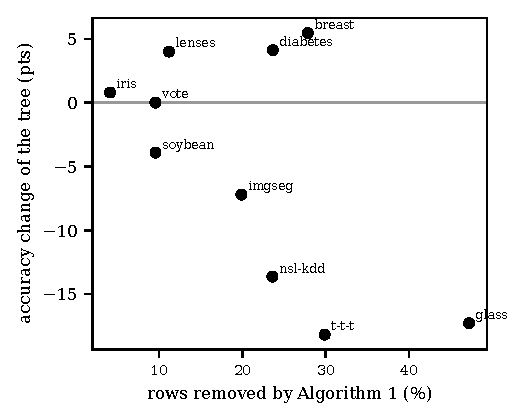
\includegraphics[width=3.4in]{figures/fig2_alg1_removal_vs_tree.pdf}
\caption{Rows Algorithm~1 removes (mean over folds and seeds, x-axis)
against the change in the downstream tree's accuracy relative to the
no-cleaning baseline (y-axis), one point per dataset. Datasets where the
filter removes a large share of rows tend to see the tree's accuracy fall.}
\label{fig:removal}
\end{figure}

% Wilcoxon signed-rank tests over the 10 datasets, Holm-adjusted within this family of 8 (n=10, low power; Demsar 2006).
\begin{table}[t]
\caption{Wilcoxon signed-rank tests over the 10 datasets (n=10 pairs unless noted; two-sided; Holm-adjusted p within this table).}
\label{tab:tests}
\centering
\small
\setlength{\tabcolsep}{3pt}
\begin{tabular}{lrrrr}
\toprule
Comparison & $W$ & $p$ & med.\ diff.\ & Holm $p$ \\
\midrule
R1 protocol A vs B, Alg1 & 0.0 & 0.002 & +11.58 & 0.016 \\
R1 protocol A vs B, Alg2 & 10.0 & 0.164 & +0.14 & 0.656 \\
E3a protocol A vs B, Alg1 & 0.0 & 0.002 & +15.52 & 0.016 \\
E3a protocol A vs B, Alg2 & 9.0 & 0.129 & +0.29 & 0.645 \\
R1 honest Alg1 vs C4.5 & 6.0 & 0.055 & -3.71 & 0.328 \\
R1 honest Alg2 vs NB & 10.0 & 0.164 & +0.65 & 0.656 \\
E9 Path 2 vs Path 1, final DT & 25.0 & 0.846 & -0.09 & 0.846 \\
E9 Path 2 vs Path 1, final NB & 17.0 & 0.322 & +0.97 & 0.656 \\
\bottomrule
\end{tabular}
\end{table}


\section{Discussion and Threats to Validity}

The central finding is a protocol effect, not an implementation bug: two
independent codebases, one built to match Farid et al.'s own tools (Weka
J48, a textbook NB on nominal columns) and one built independently
(sklearn entropy trees, one-hot attributes, a mixed-likelihood NB), agree
that fitting Algorithm~1's filter on the whole dataset before
cross-validation inflates its reported accuracy by double digits, while
fitting Algorithm~2's attribute weights the same way inflates almost
nothing. That agreement across two different attribute encodings and two
different tree implementations is evidence the effect belongs to the
algorithm's structure (Algorithm~1 removes rows that then vanish from
every test fold; Algorithm~2 only removes columns, which are never
test-fold-specific) rather than to a coding choice in either
implementation.

Several limitations bound what this replication can claim. The R1 tree is
Weka's J48, a close match to Quinlan's C4.5~\cite{quinlan1993c45}, but E3a
and E9 use scikit-learn's~\cite{pedregosa2011scikit} CART-style entropy
tree on one-hot attributes, which is not C4.5 and does not test a nominal
attribute the way the original algorithms describe; the E3a/E9 numbers
should be read as a leakage audit on a related but distinct
implementation, not as a second attempt to match the paper's Table 7--11
numbers. Ten datasets is a small sample for any between-dataset
statistical test; every Wilcoxon test in this paper has $n=10$ pairs at
most, which is why several comparisons with visually large mean
differences (for instance Algorithm~1 vs.\ C4.5 under protocol B, median
$-3.71$, raw $p=0.055$) do not survive Holm correction, and why we report
these as directional rather than as confirmed effects. All datasets come
from the paper's original 2014 benchmark, several of them (contact lenses,
iris, vote) small and decades old; nothing here speaks to how either
algorithm behaves on larger or more recent data outside this
benchmark. The seed counts (3 for R1 and E3a, 5 for E9) are smaller than
the 10 originally planned for this line of experiments, and the results
should be read as preliminary; increasing seed count would narrow the
per-arm standard deviations shown in Table~\ref{tab:e9} without changing
which comparisons are paired by dataset for the Wilcoxon tests. No
per-fold accuracy is retained in the result files produced by this
project's code, only fold-averaged, seed-averaged accuracy per dataset and
arm; a corrected resampled $t$-test that accounts for the dependence
between folds from the same dataset was therefore not computed, and we
report only the between-dataset Wilcoxon test, following
Dem\v{s}ar~\cite{demsar2006statistical}, rather than claim a test this
data cannot support.

The NSL-KDD C4.5 discrepancy (99.47\% here vs.\ 71.11\% reported) remains
unresolved and is reported plainly rather than explained away. NSL-KDD is
also the dataset with the largest number of attributes and instances in
the benchmark, and a leakage effect specific to intrusion-detection
preprocessing has been documented on it
elsewhere~\cite{bouke2023empirical}; whether the paper's 71.11\% reflects
a different data split, a different feature set, or a different intrusion
detection preprocessing step is not something this replication can
determine from the published paper alone.

This audit tests one filter design (a single NB classifier judging its
own training data) and one weighting design (inverse-square-root tree
depth); it does not test whether a consensus or ensemble
filter~\cite{brodley1999identifying}, a confidence-thresholded
filter~\cite{northcutt2021confident}, or a correction-based
alternative~\cite{jiang2024correction} would recover some of the honest
accuracy that Algorithm~1's hard deletion gives up, nor whether a
multi-view attribute weighting scheme~\cite{zhang2023multiview} would
close Algorithm~2's small remaining gap to the paper. Those are separate,
un-run experiments; this paper's claim is limited to what Algorithms~1 and
2, as specified in the 2014 paper, do under leakage-safe evaluation on
these ten datasets.

\section{Conclusion}

Replicating Farid et al.'s two decision-tree/Na\"ive-Bayes hybrids with
the paper's own components reproduces the C4.5 and NB baselines closely on
most datasets (C4.5 within 1.4 points on 7 of 9 datasets other than NSL-KDD,
NB within 2 points on 7 of 10) but does not reproduce either hybrid's reported gain
under an evaluation protocol that refits every stage inside each
cross-validation fold. Fitting Algorithm~1's noise filter once on the
whole dataset before cross-validation, rather than inside each fold,
accounts for a large and statistically significant part of the gap
between this replication and the original paper, confirmed on two
independent implementations; fitting Algorithm~2's attribute weights the
same way accounts for almost none of its own, smaller gap. Chaining the
two algorithms in either order does not recover the paper's reported
accuracy, and the order itself makes little difference. The honest result
of this replication is the protocol effect and the diagnostics behind it,
not a hybrid classifier that beats its baseline: readers who want
Algorithm~1's filtering behavior should expect it to help only where its
Na\"ive Bayes judge is already more reliable than the tree it feeds, and
to cost accuracy otherwise. All results here are preliminary, run over 3
or 5 seeds rather than the 10 planned for a final study, and are reported
with that caveat rather than rounded into a stronger claim than the data
support.


\bibliographystyle{IEEEtran}
\bibliography{references}

\end{document}
